\documentclass{article}
\usepackage[T1]{fontenc}
\usepackage{lmodern}
\usepackage{graphicx}
\usepackage{amsmath,amssymb}
\usepackage[a4paper,margin=2cm]{geometry}
\usepackage[absolute,overlay]{textpos}
\setlength{\TPHorizModule}{1mm}
\setlength{\TPVertModule}{1mm}
\usepackage[indonesian]{babel}
\usepackage{hyperref}
\setlength{\emergencystretch}{2em}
% unit: Halaman 42

\begin{document}

% === Halaman 42 (llm) ===

\section*{Output-Feedback (OFB)}

\vspace{187.11mm}

\begin{itemize}
    \item Mode $OFB$ mirip dengan mode $CFB$, kecuali $s$-bit dari hasil enkripsi antrian disalin menjadi elemen posisi paling kanan di antrian.
\end{itemize}

\vspace{60mm}

\begin{center}
    (a) Enkripsi \quad \quad \quad (b) Dekripsi
\end{center}

% deskripsi: Diagram blok proses enkripsi Output-Feedback (OFB) 8-bit yang menunjukkan aliran data melalui shift register, blok enkripsi E dengan kunci K, dan operasi XOR untuk menghasilkan ciphertext ci dari plaintext pi.
% bbox normalisasi: [0.1700, 0.3000, 0.4400, 0.9300]
\begin{textblock*}{56.70mm}(35.70mm,89.10mm)
\noindent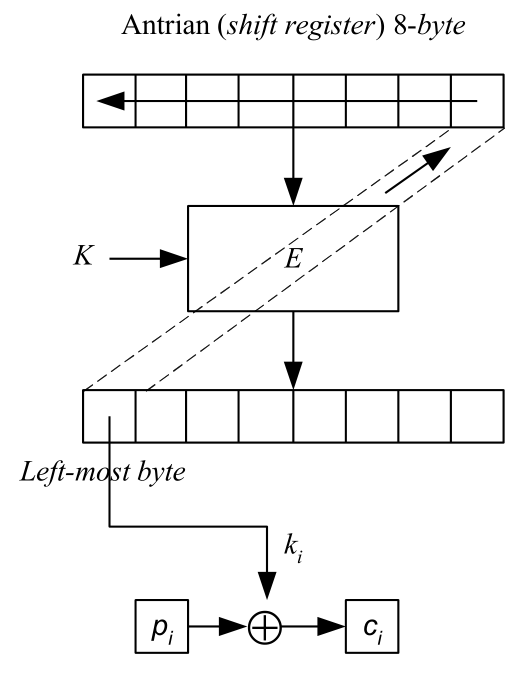
\includegraphics[width=56.70mm,height=187.11mm]{../../images/llm/page_042_img_01.png}%
\end{textblock*}

% deskripsi: Diagram blok proses dekripsi Output-Feedback (OFB) 8-bit yang menunjukkan proses yang identik dengan enkripsi, di mana ciphertext ci di-XOR dengan keystream ki untuk mendapatkan kembali plaintext pi.
% bbox normalisasi: [0.5800, 0.3000, 0.8500, 0.9300]
\begin{textblock*}{56.70mm}(121.80mm,89.10mm)
\noindent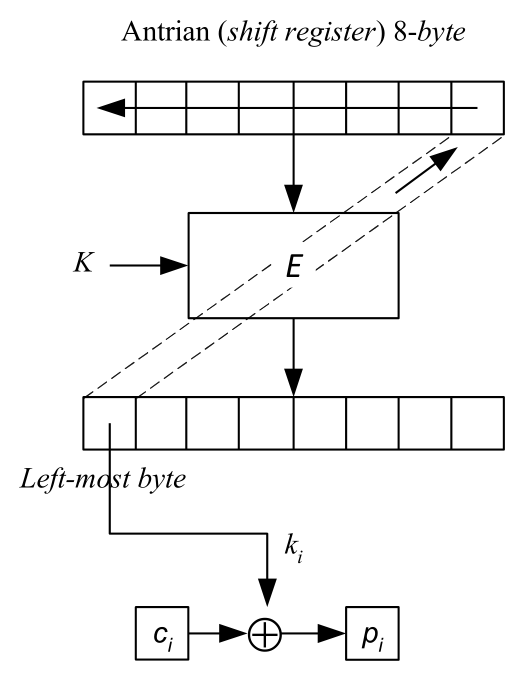
\includegraphics[width=56.70mm,height=187.11mm]{../../images/llm/page_042_img_02.png}%
\end{textblock*}

\end{document}
